% ============================================================
% ch10_error_hierarchy.tex
% Error Measurement Hierarchy
% Part of: Tetrad-Based Departure Decomposition (Jiwon Park)
% Session S9 draft — 2026-03-30
% ============================================================

\chapter{Error Measurement Hierarchy}
\label{ch:error-hierarchy}

Our goal in this chapter is to define a systematic error
budget for the species-resolved Bianchi Boltzmann solver of
Chapter~\ref{ch:results} and the multi-species $\Teff$
reduction of Chapter~\ref{ch:teff}.  The budget comprises five
levels, ordered from the microscopic state space to the
macroscopic observable, with each level measuring a distinct
source of error that can be diagnosed and controlled
independently.

The five-level structure addresses a problem that is unique to
the $\Teff$ programme.  A standard Boltzmann solver (CAMB,
CLASS) computes the CMB power spectrum from a single code path
and reports a single numerical convergence criterion
($\ell_{\rm max}$, integration tolerance).  The $\Teff$
solver, by contrast, introduces additional approximation
layers---the effective-temperature ansatz, the species-resolved
tangency diagnostic, the $\ell$-band routing, and the
nonlinear source bridge---each with its own error
characteristic.  Without a layered error budget, it is
impossible to determine where the dominant error arises and
where computational resources should be concentrated.

We define the five levels in
Sections~\ref{sec:err-state}--\ref{sec:err-observable},
discuss the cost--accuracy trade-off in
Section~\ref{sec:err-cost}, and summarise the error budget
for the Phase~1.0 solver in
Section~\ref{sec:err-phase10-budget}.


% ============================================================
\section{Level~1: State-space error}
\label{sec:err-state}
% ============================================================

The first level measures the deviation of the solver's
internal state---the PSTF multipoles of each species---from
a reference solution.


\paragraph{Definition.}

For species $s$ at conformal time $\eta$, angular multipole
$\ell$, azimuthal index $m$, and Fourier wavenumber $k$, the
state-space error is
\begin{equation}\label{eq:err-state}
\varepsilon_{\rm state}^{(s)}(\ell, \eta)
:= \frac{
  \sum_{m,k}
  \big|
    U_{\ell m k}^{(s),\text{Teff}}
    - U_{\ell m k}^{(s),\text{ref}}
  \big|^2
}{
  \sum_{m,k}
  \big|
    U_{\ell m k}^{(s),\text{ref}}
  \big|^2
}\,,
\end{equation}
where $U_{\ell m k}^{(s)}$ denotes the species multipole
(temperature, E-mode, B-mode for photons; energy and number
moments for neutrinos) and the superscripts ``Teff'' and
``ref'' denote the $\Teff$-backed solver and the reference
solution, respectively.


\paragraph{Reference solutions.}

The choice of reference depends on the background:
in the FLRW or near-isotropic limit, the reference is
the standard CAMB or CLASS output; on an anisotropic
Bianchi background, the reference is the same background
evolved with a non-$\Teff$ PSTF hierarchy (i.e.\ the full
multipole hierarchy truncated at $\ell_{\rm max}$ without
the effective-temperature ansatz).  This two-tier baseline
is essential: comparing the $\Teff$ solver against CAMB on
a strongly anisotropic background would conflate the
anisotropy-induced deviation with the $\Teff$
approximation error.


\paragraph{Band-averaged variants.}

For diagnostic purposes, we define band-averaged
state-space errors:
\begin{equation}\label{eq:err-state-band}
\varepsilon_{\rm low}^{(s)}
:= \max_{\ell \leq 2}\,
  \varepsilon_{\rm state}^{(s)}(\ell, \eta_*)\,,
\qquad
\varepsilon_{\rm mid}^{(s)}
:= \max_{3 \leq \ell \leq \ell_{\rm trans}}\,
  \varepsilon_{\rm state}^{(s)}(\ell, \eta_*)\,,
\qquad
\varepsilon_{\rm high}^{(s)}
:= \max_{\ell > \ell_{\rm trans}}\,
  \varepsilon_{\rm state}^{(s)}(\ell, \eta_*)\,,
\end{equation}
where $\ell_{\rm trans}$ is the Silk damping scale
(Section~\ref{sec:ell-band}).  The low-$\ell$ error is
the most relevant for the departure parameter pipeline,
which depends only on $D_2$ ($\ell = 2$).


\paragraph{Phase~1.0 status.}

The Phase~1.0 solver operates at $\ell_{\rm max} = 2$, so
only $\varepsilon_{\rm low}$ is defined.  In the FLRW
limit, $\varepsilon_{\rm low} = 0$ by construction (the
solver recovers $D_2 = 0$ exactly).  On the Bianchi~I
background, the oracle comparison gives
$\varepsilon_{\rm state}^{(\nu)}(2, \eta_*) \simeq 0.08$
(the $-8\%$ deviation of
Section~\ref{sec:disc-oracle}), dominated by the
analytic transfer function's missing late ISW and
neutrino stress feedback.  Phase~2.0 targets
$\varepsilon_{\rm low} < 0.02$ through self-consistent
Poisson (Section~\ref{sec:phase20}).


% ============================================================
\section{Level~2: Source-translation error}
\label{sec:err-source}
% ============================================================

The second level measures the accuracy of the $\Teff$
nonlinear source bridge---the map from the angular
temperature field $\Theta_s(\hat{e})$ to the Thomson
scattering source that enters the Boltzmann hierarchy.


\paragraph{Definition.}

The source-translation error for the photon Thomson source is
\begin{equation}\label{eq:err-Th}
\varepsilon_{\rm Th}
:= \frac{
  \big|
    I_{ab}^{\rm ref}
    - c_\xi\,
      \langle \Theta_\gamma^4\,
      \hat{e}_{\langle a}\hat{e}_{b\rangle}
      \rangle_\Omega
  \big|
}{
  \big| I_{ab}^{\rm ref} \big|
}\,,
\end{equation}
where $I_{ab}^{\rm ref}$ is the photon anisotropic stress
computed from the full Boltzmann hierarchy (without the
$\Teff$ ansatz) and the $\Theta^4$ term is the $\Teff$
moment-map reconstruction
(Eq.~\ref{eq:exact-bridge}).  A companion diagnostic
compares against the linearised bridge:
\begin{equation}\label{eq:err-Th-lin}
\varepsilon_{\rm Th}^{\rm lin}
:= \frac{
  \big|
    I_{ab}^{\rm ref}
    - 4\,c_\xi\,\Theta^{(\gamma)}_{ab}
  \big|
}{
  \big| I_{ab}^{\rm ref} \big|
}\,.
\end{equation}
The difference
$\varepsilon_{\rm Th}^{\rm lin} - \varepsilon_{\rm Th}$
isolates the contribution of the nonlinear ($\Theta^4$
vs.\ $4\Theta$) correction.  At moderate dipole amplitudes
($A \sim 10^{-2}$), the linear bridge can err by up to
$52\%$, while the nonlinear bridge maintains
$\varepsilon_{\rm Th} < 1\%$---a demonstration that the
$\Theta^4$ moment map provides a qualitatively superior
source translation even when the dipole is not small.


\paragraph{Phase~1.0 status.}

In the Phase~1.0 solver, the Thomson source uses the
linearised form (Eq.~\ref{eq:Thomson-damping}) because the
shear-driven quadrupole is the dominant source and the
dipole is small ($A \sim \beta \sim 10^{-3}$).  The
source-translation error is therefore
$\varepsilon_{\rm Th}^{\rm lin} \sim 10^{-3}$, consistent
with the second-order estimate of
Section~\ref{sec:quadratic-sources}.  The nonlinear bridge
becomes essential only when the dipole amplitude exceeds
$\sim\!10^{-2}$, which lies in the nonperturbative regime
(Section~\ref{sec:nonperturbative}).


% ============================================================
\section{Level~3: Adequacy certificate}
\label{sec:err-adequacy}
% ============================================================

The third level is not an error per se but a
\emph{certificate}: a bound on the observable-level
representation error, computed from the tangency diagnostic
and the Jacobian condition number.


\paragraph{Definition.}

For species $s$, the adequacy certificate is
\begin{equation}\label{eq:err-adequacy}
\Delta_{\rm obs}^{(s),\text{bound}}
:= \frac{C(\xi_s, L_s)}
        {\sigma_{\min}(J_s)}\,
  D_{s,\geq 2}\,,
\end{equation}
where $C(\xi_s, L_s)$ is a constant that depends on the
quantum statistics and truncation level,
$\sigma_{\min}(J_s)$ is the smallest singular value of the
species Jacobian $J_s$
(Eq.~\ref{eq:chain-rule}), and $D_{s,\geq 2}$ is the
tangency diagnostic
(Eq.~\ref{eq:D-diagnostic}).  The certificate guarantees
\begin{equation}\label{eq:adequacy-bound}
\Delta_{\rm obs}^{(s),\text{actual}}
\leq \Delta_{\rm obs}^{(s),\text{bound}}
+ O\big(D_{s,\geq 2}^2\big)\,.
\end{equation}


\paragraph{Interpretation.}

The certificate is conservative: the bound overestimates
the actual error because it uses the worst-case direction
of the tangency residual.  The tightness ratio
\begin{equation}\label{eq:tightness}
\rho_s
:= \frac{\Delta_{\rm obs}^{(s),\text{actual}}}
        {\Delta_{\rm obs}^{(s),\text{bound}}}
\end{equation}
quantifies the conservatism.  For representative
configurations [CITATION NEEDED: Teff Paper~IV],
$\rho_s \sim 0.003$---the bound is never violated but is
three orders of magnitude loose.  The looseness is
acceptable for qualitative regime separation (identifying
when the $\Teff$ closure needs upgrading) but
insufficient for precision error propagation, which
requires the actual observable error (Level~5).


\paragraph{Scope limitation.}

The adequacy certificate is a \emph{local} bound: it
certifies the reconstruction quality at a single
conformal time $\eta$, not over the full line-of-sight
integration.  Cumulative error over cosmological
timescales is not bounded by the certificate
(Section~\ref{sec:limit-recovery}, ``Not established''
item~4).  The certificate should therefore be evaluated
at multiple epochs and combined with the observable error
(Level~5) for end-to-end accuracy assessment.


\paragraph{Phase~1.0 status.}

For neutrinos, $D_{\nu,\geq 2} = 0$ exactly
(free-streaming species have no collision source), so the
adequacy certificate is identically zero.  For photons
before recombination, $D_{\gamma,\geq 2}$ is nonzero but
suppressed by Thomson damping ($D_{\gamma,\geq 2} \sim
\sigma_{ab}/\dot{\tau} \sim 10^{-8}$), giving a certificate
$\Delta_{\rm obs}^{(\gamma)} \lesssim 10^{-8}$.  The
$\Teff$ closure is therefore certified adequate at all
epochs probed by the Phase~1.0 solver.


% ============================================================
\section{Level~4: Ladder-specific adequacy}
\label{sec:err-ladder}
% ============================================================

The fourth level tracks the error introduced by the
adaptive $\ell$-band routing of
Section~\ref{sec:ell-band}, which assigns different
computational strategies to different angular scales.


\paragraph{Definition.}

Three diagnostics measure the ladder-specific adequacy.
The deceleration-parameter adequacy is
\begin{equation}\label{eq:err-Dq}
\Delta_q^{(s)}
:= \left|
  q^{(s),\text{Teff}}_0
  - q^{(s),\text{ref}}_0
\right|\,,
\end{equation}
where $q_0$ is the present-epoch deceleration parameter
contributed by species $s$.  The number-to-energy ratio
adequacy is
\begin{equation}\label{eq:err-DNE}
\Delta_{N/E}^{(s)}
:= \left|
  \frac{j_s^a}{q_s^a}\bigg|_{\rm Teff}
  - \frac{j_s^a}{q_s^a}\bigg|_{\rm ref}
\right|\,,
\end{equation}
measuring the accuracy of the two-field reconstruction of
the number-to-energy flux ratio
(Proposition~\ref{prop:flux-independence}).  The moment
residual is
\begin{equation}\label{eq:err-Rmom}
\mathcal{R}_{A_k}^{(s),\text{mom}}
:= \left|
  m_s^{(k),\text{Teff}}
  - m_s^{(k),\text{ref}}
\right|\,,
\end{equation}
measuring the accuracy of the $k$-th observable moment
(Eq.~\ref{eq:obs-vector}).


\paragraph{Role in the adaptive strategy.}

These diagnostics are not post-hoc quality measures but
runtime decision variables.  In the Phase~4.0 adaptive
ladder (Section~\ref{sec:solver-programme}), the
$\ell$-band router evaluates $\Delta_q$ and
$\Delta_{N/E}$ at each epoch boundary and upgrades the
species representation (from one-field to two-field, or
from the $\Teff$ closure to the full PSTF hierarchy) when
the diagnostics exceed their tolerances.  The upgrade is
conservative by design: over-upgrading (using a more
expensive representation when a cheaper one would suffice)
wastes computational resources but does not introduce
error, while under-upgrading produces inaccurate results.
The frozen-rung time-slab strategy---upgrading only at
epoch boundaries rather than at every time step---avoids
the numerical instability that can arise from frequent
representation switching.


\paragraph{Phase~1.0 status.}

The Phase~1.0 solver does not implement adaptive $\ell$-band
routing; it operates at a fixed truncation
$\ell_{\rm max} = 2$ with a fixed species configuration
(one-field photons, two-moment neutrinos).  The
ladder-specific diagnostics are therefore not evaluated at
runtime.  The P1-3 discrepancy between the polarised and
unpolarised code paths ($3\%$ in $D_2$;
Section~\ref{sec:solver-performance}) is a surrogate
indicator: it measures the error introduced by the choice
of whether to include E-mode polarisation in the hierarchy,
which is the simplest form of a representation-switching
decision.


% ============================================================
\section{Level~5: Observable error}
\label{sec:err-observable}
% ============================================================

The fifth and final level measures the deviation of the
solver's output in the space of observables---the CMB power
spectra and spherical-harmonic coefficients---from the
reference solution.


\paragraph{Definition.}

The $a_{\ell m}$ error is
\begin{equation}\label{eq:err-alm}
\varepsilon_{a_{\ell m}}
:= \frac{
  \big|
    a_{\ell m}^{\rm Teff}
    - a_{\ell m}^{\rm ref}
  \big|
}{
  \big| a_{\ell m}^{\rm ref} \big|
}\,.
\end{equation}
The angular power spectrum error is
\begin{equation}\label{eq:err-Cl}
\varepsilon_{C_\ell}
:= \frac{
  \big|
    C_\ell^{\rm Teff}
    - C_\ell^{\rm ref}
  \big|
}{
  \big| C_\ell^{\rm ref} \big|
}\,.
\end{equation}
On anisotropic backgrounds, the off-diagonal covariance
$\langle a_{\ell m}\,a_{\ell' m'}^* \rangle$ is generically
nonzero (the Bianchi shear couples different $\ell$ and $m$),
and the covariance error
\begin{equation}\label{eq:err-cov}
\varepsilon_{\rm cov}
:= \frac{
  \big|
    \langle a_{\ell m}\,a_{\ell' m'}^* \rangle_{\rm Teff}
    - \langle a_{\ell m}\,a_{\ell' m'}^* \rangle_{\rm ref}
  \big|
}{
  \big|
    \langle a_{\ell m}\,a_{\ell' m'}^* \rangle_{\rm ref}
  \big|
}
\end{equation}
must be tracked for the direction-dependent programme
(Section~\ref{sec:phase30}).  The covariance error
captures the $\ell$--$\ell'$ mode mixing induced by
the background anisotropy, which is invisible to the
isotropic power spectrum $C_\ell$.


\paragraph{Relation to the Bayes factor.}

The Bayes factor $\ln \mathcal{B}$ computed by the
departure pipeline (Chapter~\ref{ch:results}) is a
functional of the likelihood, which in turn depends on
$D_2 \propto C_2$.  The observable error
$\varepsilon_{C_2}$ therefore propagates directly into the
evidence:
\begin{equation}\label{eq:err-lnB}
\delta(\ln \mathcal{B})
\sim \frac{\partial \ln \mathcal{B}}
          {\partial \ln D_2}\,
     \varepsilon_{C_2}\,.
\end{equation}
For the VER06 pipeline, the sensitivity
$\partial \ln \mathcal{B} / \partial \ln D_2 \sim
O(10)$, so an observable error of $\varepsilon_{C_2}
\sim 0.01$ ($1\%$) translates to
$\delta(\ln \mathcal{B}) \sim 0.1$---comparable to the
statistical uncertainty $\pm 0.07$ of the production
evidence.  The Phase~2.0 target
$\varepsilon_{C_2} < 0.02$ therefore ensures that the
systematic error from the solver is subdominant to the
statistical error of the inference.


\paragraph{Phase~1.0 status.}

The Phase~1.0 solver computes $D_2$ (proportional to
$C_2$ at $\ell = 2$) but does not compute the full
$C_\ell$ spectrum or $a_{\ell m}$.  The observable
error at $\ell = 2$ is $\varepsilon_{C_2} \simeq 0.08$
(the oracle deviation), which is the dominant error in
the current budget.  Phase~3.0 extends the observable
error to the full $a_{\ell m}$ spectrum, targeting
$\varepsilon_{a_{\ell m}} < 0.01$ at $\ell \leq 30$.


% ============================================================
\section{Cost--accuracy trade-off}
\label{sec:err-cost}
% ============================================================

The $\Teff$ programme's computational advantage lies in
selective upgrading: applying expensive representations
only where the diagnostics demand it, rather than
uniformly across all species and angular scales.  The
cost--accuracy trade-off quantifies this advantage.


\paragraph{Cost metrics.}

Two cost metrics are tracked alongside the error budget:
the wall-clock time per likelihood evaluation,
$\mathcal{C}_{\rm wall}$, and the memory footprint per
evaluation, $\mathcal{C}_{\rm mem}$.  For the Phase~1.0
solver, $\mathcal{C}_{\rm wall} = 420$~ms and
$\mathcal{C}_{\rm mem} \sim 50$~MB.  For comparison,
AniCLASS achieves $\mathcal{C}_{\rm wall} \sim 1$~s per
evaluation at $\ell_{\rm max} = 30$ in the linearised
regime.


\paragraph{Pareto frontier.}

The Pareto frontier in the
$(\mathcal{C}_{\rm wall}, \varepsilon_{\rm obs})$ plane
delineates the set of configurations that cannot be
improved in one dimension without degrading the other.
The $\Teff$ programme's adaptive strategy is designed to
operate near this frontier: the low-$\ell$ band uses
exact quadrature (high accuracy, moderate cost), the
mid-$\ell$ band uses the $\Teff$ ladder with selective
upgrading (controlled accuracy, reduced cost), and the
high-$\ell$ band uses the standard PSTF hierarchy
(baseline accuracy, baseline cost).  The selective-upgrading
result---that targeting upgrades where
$D_{s,\geq 2} > \varepsilon_{\rm thr}$ outperforms
uniform high-resolution computation in cost--accuracy
trade-off---is the operational vindication of the $\Teff$
approach.

For the scalar-amplitude pipeline, the Pareto frontier is
trivially achieved: only $\ell = 2$ matters, the
$\Teff$ closure is exact for the dominant neutrino
channel, and the evaluation cost ($420$~ms) is set by
the hierarchy ODE integration rather than by the
closure strategy.  The frontier becomes non-trivial for
the direction-dependent programme, where the full
$a_{\ell m}$ spectrum at $\ell \leq 30$ requires
$\sim\!10^3$ multipoles and the cost savings from
selective upgrading can reach an order of magnitude.


% ============================================================
\section{Massive neutrino as a systematic}
\label{sec:massive-neutrino-systematic}
% ============================================================

The baseline error ledger in this chapter treats the neutrino sector as
exactly massless.  That is the correct LB-1 anchor, but it is not the
final systematic floor: Planck~2018 allows a non-zero summed neutrino
mass at the sub-eV level \cite{Planck2018VI}.  FB-9 therefore adds a
separate massive-neutrino branch whose purpose is not to reopen the
entire solver programme, but to quantify how a finite
$\Sigma m_\nu$ perturbs the background equation of state and the
free-streaming scale while preserving the massless anchor exactly when
$\Sigma m_\nu = 0$.

\subsection{FB-9.1: phase-space grid}

The positive-mass branch evaluates the usual collisionless Fermi-Dirac
integrals on a deterministic Gauss-Laguerre grid with $N_q = 15$,
matching the standard CLASS/CAMB non-cold-relic convention at the level
needed for a frozen-oracle regression \cite{LesgourguesTram2011}.  The
important point for the hierarchy is not the quadrature family by
itself, but the fact that the same fixed momentum support is reused
everywhere: background density, pressure, the effective streaming
velocity, and the associated regression fixtures all derive from the
same $(q_i, w_i)$ table.  This removes one hidden degree of freedom from
the systematic budget.

\subsection{FB-9.2: background thermodynamics}

The massive-neutrino background replaces the exact radiation law
$\rho_\nu \propto a^{-4}$ by the standard interpolation between the
relativistic and non-relativistic limits
\cite{MaBertschinger1995,LesgourguesTram2011}.  Figure
~\ref{fig:massive-nu-nr-transition} shows the representative
$\Sigma m_\nu = 0.12\,\mathrm{eV}$ turnover: the scaled density rises
above its relativistic plateau while the scaled pressure drops away from
the $w = 1/3$ branch.  The transition is mild on the expansion history
but it is a real systematic in any species-resolved solver, because it
changes the neutrino sector from a pure radiation fluid into a
time-dependent effective fluid.

\begin{figure}[t]
\centering
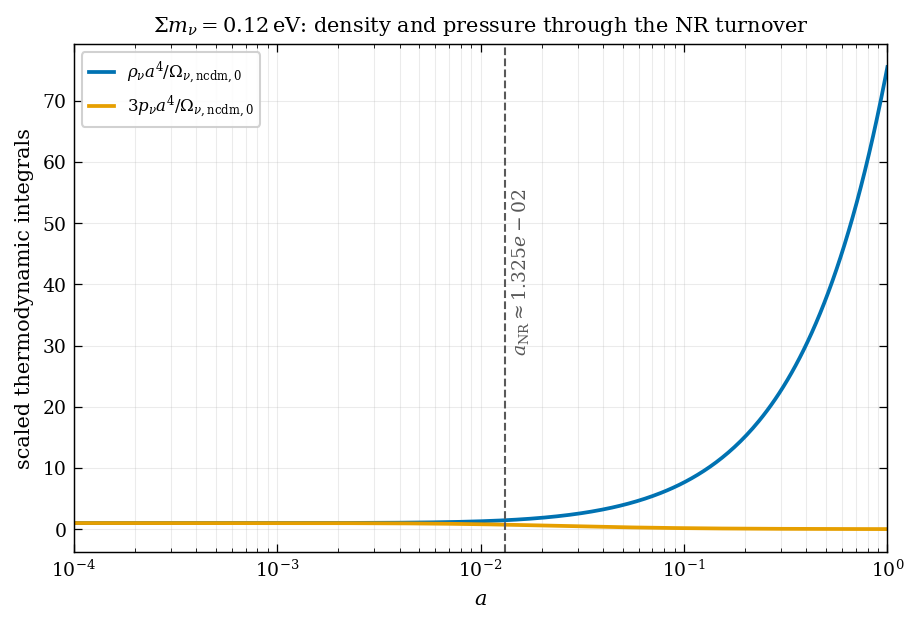
\includegraphics[width=0.78\columnwidth]{../../figures/physics_gallery/15_massive_neutrino/02_rho_p_NR_transition.png}
\caption{FB-9.2 massive-neutrino background transition for
  $\Sigma m_\nu = 0.12\,\mathrm{eV}$.  The vertical marker denotes the
  nominal non-relativistic turnover scale $a_{\rm NR}$.}
\label{fig:massive-nu-nr-transition}
\end{figure}

\subsection{FB-9.3: registry integration and the zero-mass anchor}

The systematic is introduced through the existing neutrino registry
slot, not through a new species label.  This matters for auditability:
all downstream code continues to ask for ``the neutrino background'',
while the factory dispatch decides whether that slot is massless or
massive.  The corresponding regression pin is stronger than a numerical
agreement test: with $\Sigma m_\nu = 0$ the hierarchy driver and the
full \texttt{bass/tsc} suite remain byte-identical to the LB-1 massless
path.
That short-circuit turns the massive-neutrino systematic into an
explicit opt-in perturbation rather than an ambient code-path drift.

\subsection{FB-9.4: free streaming and power suppression}

Once the neutrino species is massive, the relevant control parameter is
the free-streaming scale $k_{\rm fs}(a)$ rather than the purely
radiation-like ``free'' neutrino hierarchy.  FB-9 wires the hierarchy
through an effective $q/\epsilon$ streaming factor and recovers the
standard $k_{\rm fs}$ scaling to within the audit tolerance
\cite{LesgourguesTram2011,HuEisensteinTegmark1998}.  In practical terms,
the systematic is concentrated on modes with $k \gtrsim k_{\rm fs}$,
where the leading-order matter-power response approaches the familiar
$-8 f_\nu$ suppression.  The result is conceptually simple: the massive
neutrino is not a new dynamical sector, but a controlled deformation of
the neutrino hierarchy with a known large-$k$ footprint.

% ============================================================
\section{Phase~1.0 error budget summary}
\label{sec:err-phase10-budget}
% ============================================================

We summarise the error budget for the Phase~1.0 solver
and identify the dominant error at each level.

\begin{center}
\setlength{\tabcolsep}{5pt}
\begin{tabular}{llll}
\hline\hline
Level & Diagnostic & Phase~1.0 value & Dominant source \\
\hline
1. State-space
  & $\varepsilon_{\rm state}^{(\nu)}(\ell{=}2)$
  & $0.08$
  & Analytic $\Psi(k,\eta)$ \\[3pt]
2. Source-translation
  & $\varepsilon_{\rm Th}^{\rm lin}$
  & $\sim 10^{-3}$
  & Linearised Thomson \\[3pt]
3. Adequacy certificate
  & $\Delta_{\rm obs}^{(\gamma)}$
  & $\lesssim 10^{-8}$
  & Thomson suppression \\[3pt]
  & $\Delta_{\rm obs}^{(\nu)}$
  & $= 0$ (exact)
  & Free-streaming \\[3pt]
4. Ladder-specific
  & not evaluated
  & ---
  & Fixed truncation \\[3pt]
5. Observable
  & $\varepsilon_{C_2}$
  & $0.08$
  & $= \varepsilon_{\rm state}$ \\
\hline\hline
\end{tabular}
\end{center}

The dominant error is at Level~1 (state-space), arising
from the analytic gravitational potential.  The $\Teff$
closure itself contributes negligibly: the adequacy
certificate is $\leq 10^{-8}$ for photons and exactly
zero for neutrinos.  The source-translation error is
$\sim 10^{-3}$, three orders of magnitude below the
state-space error.  The error budget confirms that the
$\Teff$ approximation is not the bottleneck---the
gravitational potential is---and that Phase~2.0
(self-consistent Poisson) is the correct next step.

The error hierarchy also reveals a structural asymmetry
between species.  The neutrino sector contributes
$98.4\%$ of $D_2$ but introduces zero $\Teff$ error
(Levels~2--3), because free-streaming neutrinos reside
exactly on the $\Teff$ manifold.  The photon sector
contributes $1.6\%$ of $D_2$ and carries the only
nonzero $\Teff$ error, but this error is suppressed by
Thomson damping to a level that is irrelevant at any
foreseeable precision.  The $\Teff$ closure is therefore
not merely adequate but structurally optimal for the
species composition of the standard cosmological model:
the dominant species is exactly closed, and the
subdominant species is over-damped.

Before closing this chapter, we note that the five-level
hierarchy is designed to be extensible.  As the solver
programme advances through Phases~2.0--5.0
(Section~\ref{sec:solver-programme-ch9}), each level
acquires additional diagnostics---self-consistent
Poisson residuals at Level~1, nonlinear Thomson bridge
accuracy at Level~2, AniCLASS $a_{\ell m}$ comparison
at Level~5---without changing the overall structure.
The hierarchy is a framework for error accounting, not a
fixed set of numbers.
